\subsubsection{Hybrid Model}
\label{caseStudyHybridModel}
	\begin{enumerate}
	\item Trajectories are defined for right to left lane switch and left to right lane switch.
	\item Hybrid system modes are described by drive forward and lane change.
	\begin{enumerate}
		\item Lane change is hierarchical and has sub-modes, right to left, straight, and left to right.
		\item Each submode has same dynamics but implements a different motion primitive.
	\end{enumerate}

		\begin{figure}[tb]
			\label{fig:hybrid}
			\centering
			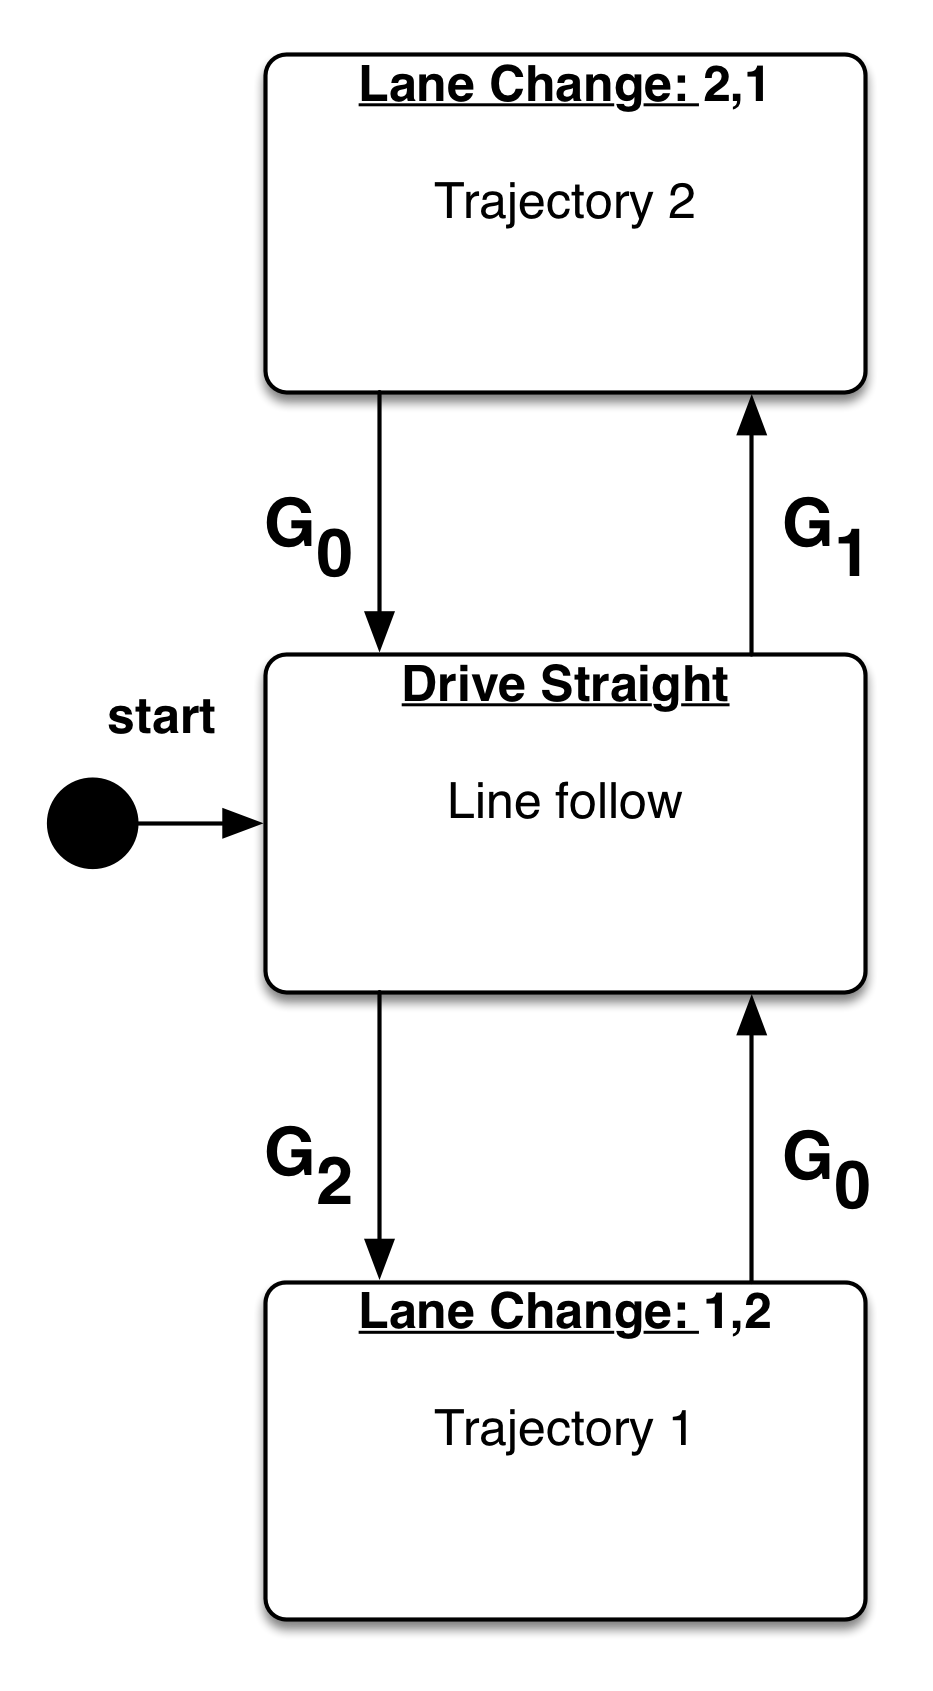
\includegraphics[scale=.5]{hybrid.png}
			\caption{Hybrid automata describing lane change}
		\end{figure}
	\item Fig.\ref{fig:hybrid} describes the system.
	\item[] \(G_1\) and \(G_2\) If there is a vehicle detected in the current lane traveling at a velocity less than the target vehicle's velocity, and there exists another lane which has the same direction of travel as the current lane, and the reachable set of the target vehicle executing a motion primitive for a lane change does not intersect with any other vehicle in the scenario, transition to the lane change mode.
	\item[] \(G_0\) If lane change motion primitive is complete, transition back to the follow lane mode.
		\end{enumerate}
		
Final control equations generate inputs for the plant which represent longitudinal acceleration and the rate of change of the steering angle:
\begin{equation}
\begin{aligned}
v_w=k_1(cos{(\Psi_d)}(s_{y,d}-s_y-w_y)\\
-sin{(\Psi_d)}(s_{x,d}-s_x-w_x)\\ 
+k_2(\Psi_d-\Psi-w_{\Psi}) \\
+k_3(\dot{\Psi_d} -\dot{\Psi}-w_{\psi})\\
-k_4(\delta-w_{\delta})
\end{aligned}
\end{equation}
\begin{equation}
\begin{aligned}
a_x=k_5(cos{(\Psi_d)}(s_{x,d}-s_x-w_x)\\
+sin{(\Psi_d)}(s_{y,d}-s_y-w_y)\\
+k_6(v_d-v-w_v)
\end{aligned}
\end{equation}
ADD guard condition information